\begin{figure}
    \begin{center}
    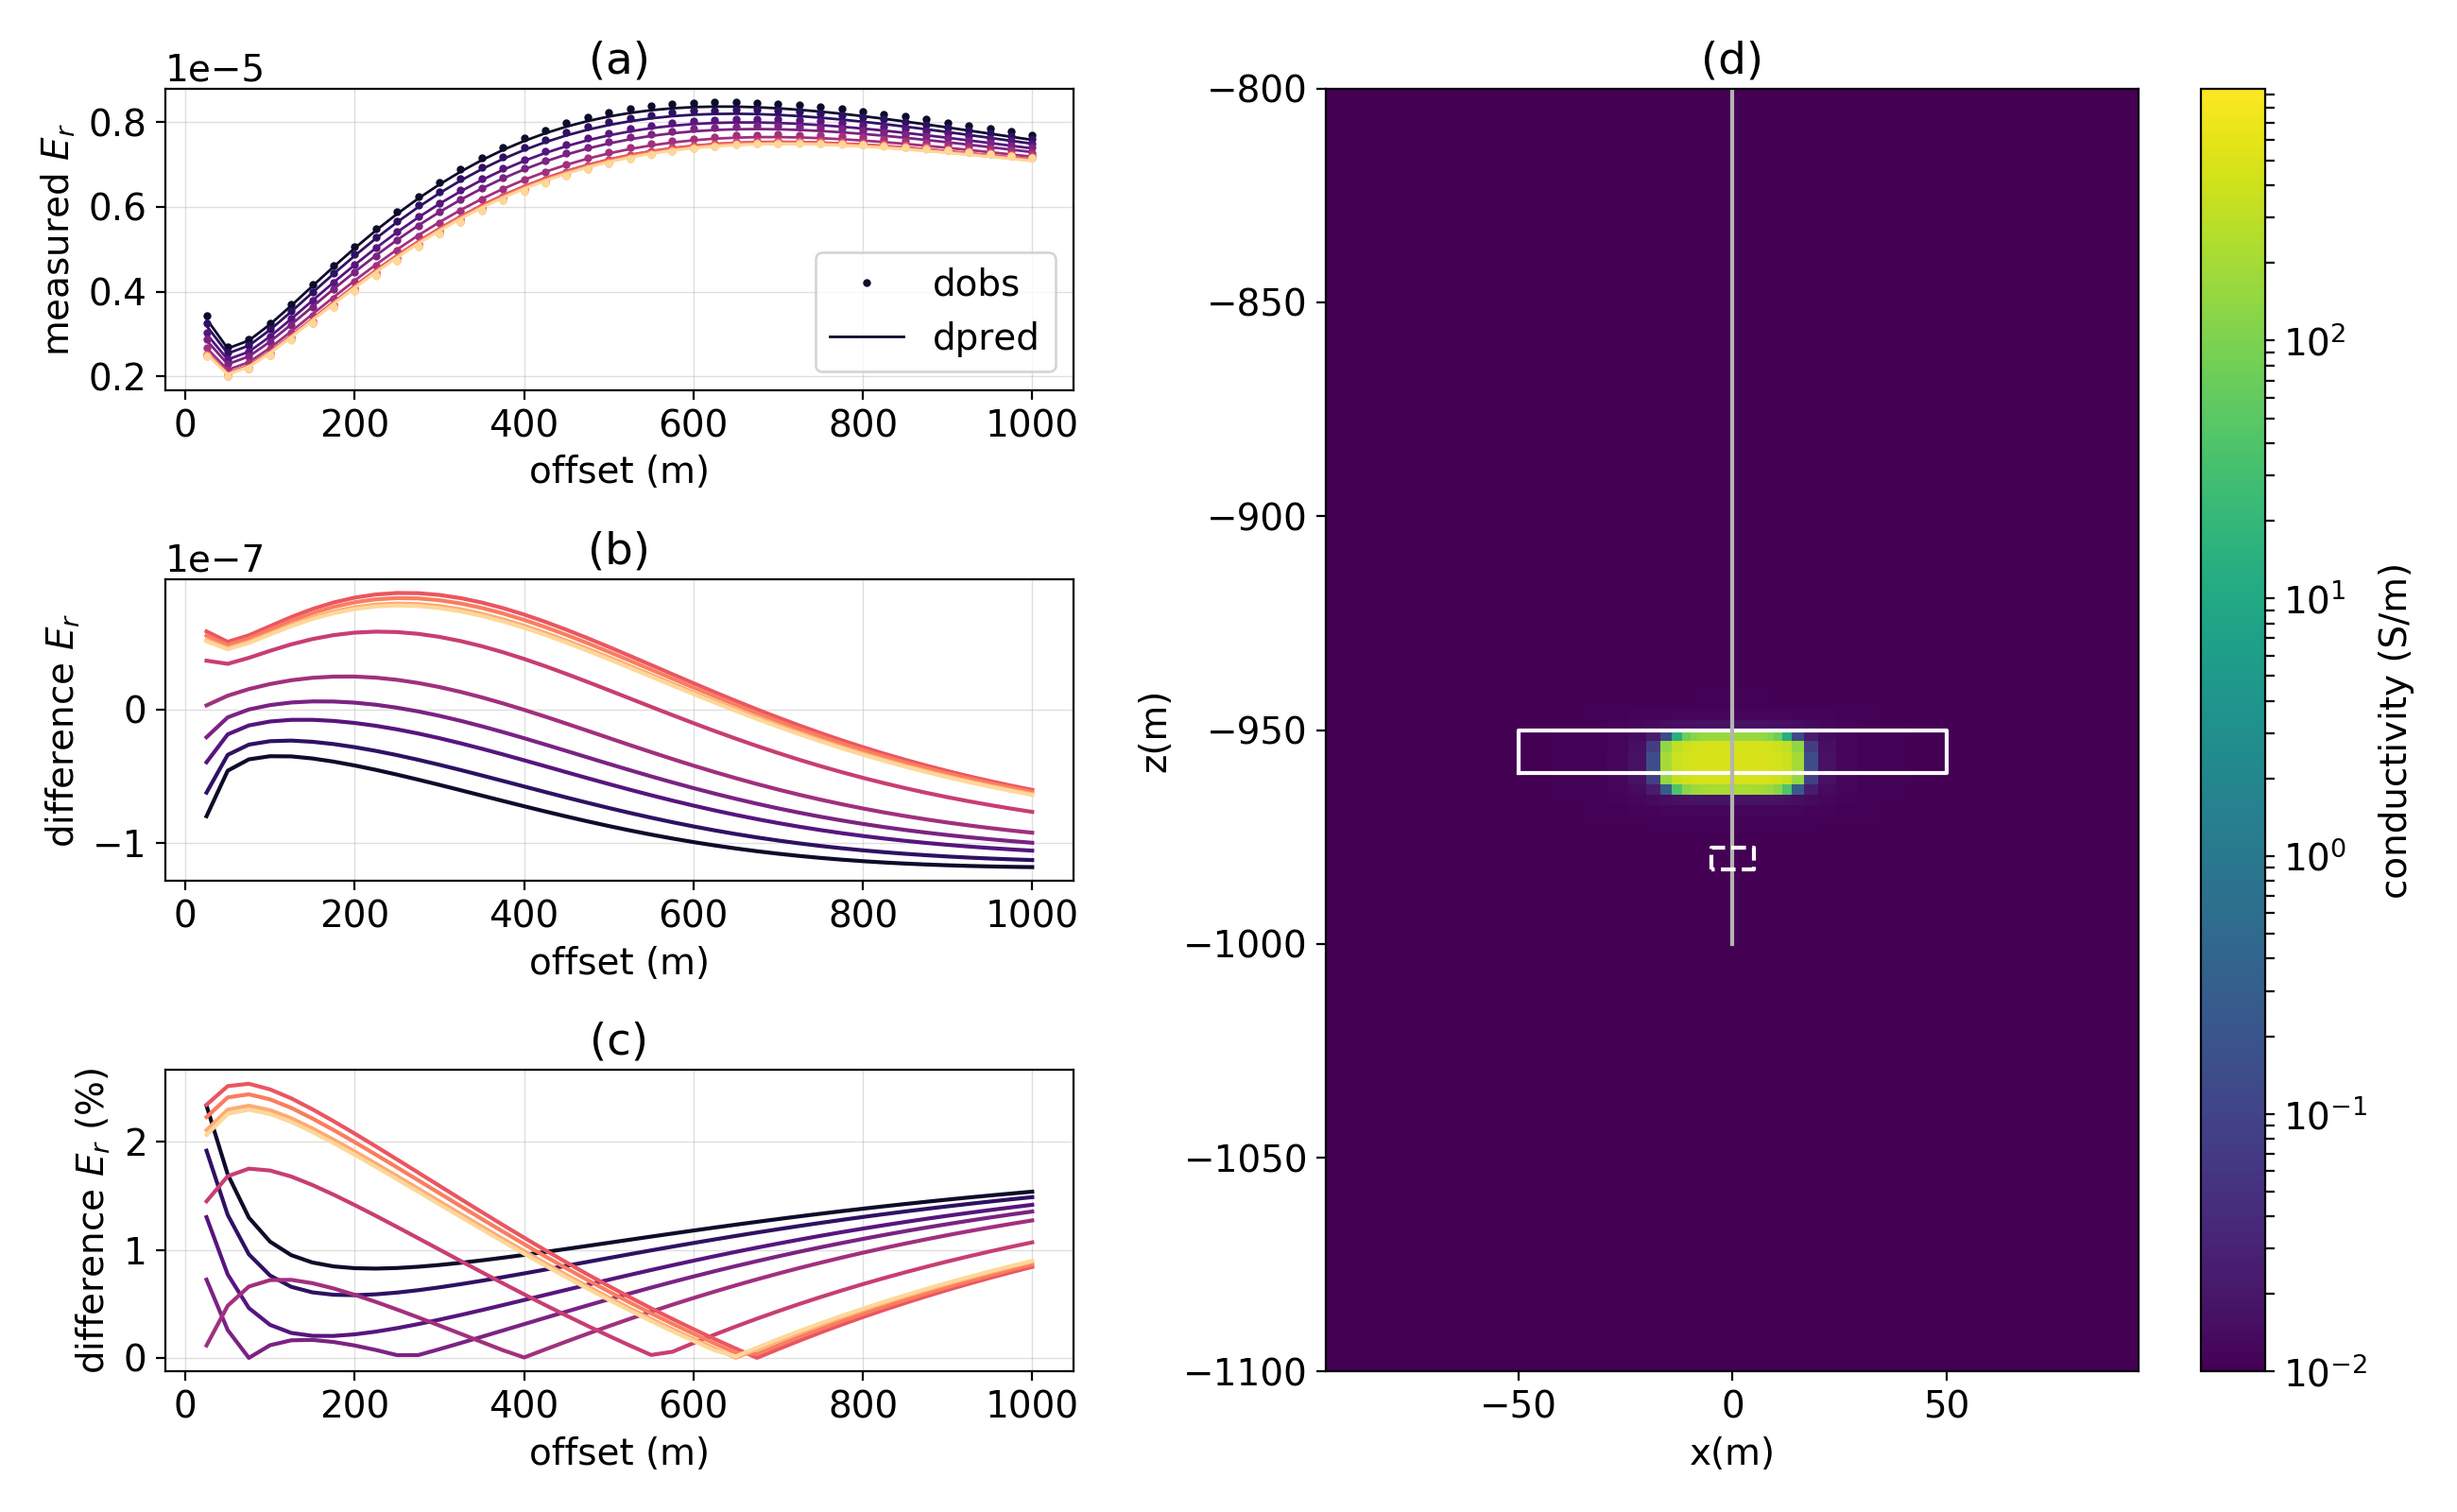
\includegraphics[width=1\textwidth]{figures/inversion/parametric_voxel1.png}
    \end{center}
\caption{
    Parametric inversion result for a starting model
    centered at 980m depth with a thickness of 5m and a radius of 10m. The initial background
    conductivity is $10^{-2}$ S/m and the initial conductivity of the target is $3\times10^{-2}$ S/m.
    The geometry of the starting model is shown by the white dashed-lines and the
    true model is shown by the solid white outline. The inversion reached a $\chi$-factor < 0.05
    and took 8 iterations.
\label{fig:parametric_voxel1}
\end{figure}
